\chapter{Numerical results}
\label{chap:results}


\prettyref{chap:patching} and \prettyref{chap:MPOcontr} introduced our \emph{patched QTCI} and \emph{patched MPO–MPO contraction} algorithms in detail. By extending the state-of-the-art implementation of the QTCI algorithm, we have implemented a \textit{divide‐and‐conquer} version of TCI that targets scenarios in which the standard routine may struggle.

In this chapter we first present representative benchmarks (\prettyref{sec:2DGreen} and \prettyref{sec:benchmarkMPOMPOContr}) that highlight the performance of the new routines. We then apply them to two physics problems that have previously posed computational bottlenecks: the two–dimensional Hubbard model (\prettyref{sec:bubbleCalc}) and the single‐impurity Anderson model (Sec.~\ref{sec:patchBSE}). Both cases were recently addressed with QTCI or patched quantics SVD–based tensor trains approaches \cite{Hiroshi2023,Rohshap2025}. Our patched QTCI method complements and extends those efforts, demonstrating improved efficiency on the same benchmark tasks.

Our calculations are constructed on the alreadymature $\julia$ packages \texttt{TensorCrossInterpolation.jl} \cite{TensorCrossInterpolation.jl} and \texttt{QuanticsTCI.jl} \cite{tensor4all.org}, which we have extended with the additional features required for the present applications.

\section{Approximation of 2D Green's functions}
\label{sec:2DGreen}

We begin with the toy Green’s function  

\begin{equation}
  G(\mathbf{k})
  \;=\;
  \frac{1}
       {\;\omega+\mu-\varepsilon_{\mathbf{k}}+i\delta\,},
  \label{eq:2DGreen}
\end{equation}

where the non-interacting dispersion is taken as
\(\varepsilon_{\mathbf{k}}=-2\cos k_{x}-2\cos k_{y}\)  
and we set the chemical potential to \(\mu=0\).
\prettyref{eq:2DGreen} is patterned after the Matsubara Green’s function of the two-dimensional Hubbard model at finite temperature
\cite{Mahan2000},

\begin{equation}
  G(i\nu,\mathbf{k})
  \;=\;
  \frac{1}
       {\,i\nu+\mu-\varepsilon_{\mathbf{k}}-\Sigma(i\nu,\mathbf{k})},
\end{equation}

with two deliberate simplifications:
\(\omega\) plays the rôle of the (real) self-energy
\(\Sigma\), while \(\delta\) mimics the Matsubara frequency
\(\nu=(2n+\xi)\pi/\beta\) ($\xi=0,1$ for bosons and fermions) and thus encodes the temperature.
Accordingly we treat \(\omega\) as a fixed input—one may think of it as the self-energy obtained from the previous Dyson iteration—whereas \(\delta\) is varied to emulate different temperatures.

The figure below shows a density plot of
\(\operatorname{Re}G(\mathbf{k})\) for the representative choice
\(\omega=10^{-1}\):

\begin{figure}[ht!]
    \centering
    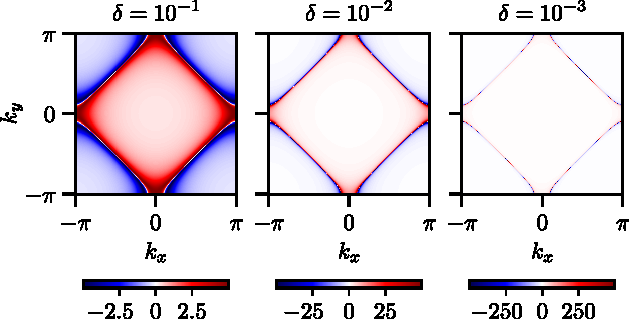
\includegraphics{figures/realGreenHeatmap.pdf}
    \caption{Heatmap of the real part of the Green's function in \prettyref{eq:2DGreen}, $\text{Re}\left(G(\bk)\right)$ for different values of $\delta$ and fixed $\omega=10^{-1}$. }
    \label{fig:realGreenHeatmap}
\end{figure}

\prettyref{fig:realGreenHeatmap} shows that the parameter \(\delta\) controls how sharply the Green’s function is localised: as \(\delta\to 0\) the poles narrow and \(G(\mathbf{k})\) becomes increasingly singular.  This makes the function an ideal testbed for patched QTCI.

We discretise \(G(\mathbf{k})\) by quantics rebasing,  
\begin{equation}
  G(\bk)
  \;\longrightarrow\;
  G_{\bsigma} = G\!\bigl(\bk(\bsigma)\bigr),
\end{equation}
with bit string
\(\boldsymbol{\sigma}=(\sigma_{1},\dots,\sigma_{\mathcal R})\) in the fused
ordering, or \(\boldsymbol{\sigma}=(\sigma_{x1},\dots,\sigma_{y\mathcal R})\) in the interleaved ordering.  
Throughout we use \(\mathcal R=15\) bits per \(\bk\)-component.

After setting a patch bond–dimension cap \(\chi_{\text{patch}}\) and a global tolerance \(\tau=10^{-7}\), we monitor convergence of pQTCI via the pointwise error
\begin{equation}
  \varepsilon(\mathbf{k})
  = \log_{10}\!
      \frac{\bigl|\operatorname{Re}\widetilde G(\mathbf{k})
                -\operatorname{Re}G(\mathbf{k})\bigr|}
           {\;\|\operatorname{Re}\widetilde G\|_{\infty}},
  \label{eq:localError2DGreen}
\end{equation}
where \(\|\operatorname{Re}\widetilde G\|_{\infty}\) is the maximum of \(|\operatorname{Re}\widetilde G|\) over all sampling points \(\bk(\bsigma)\) used in every patch \(\operatorname{Re} \widetilde{G}^{p_1,\dots,p_{\bar\ell}}\) produced by the patched QTCI routine.

\prettyref{fig:2DGreenErrorHeatmap} compares the patched QTCI approximation with the exact real part of the Green’s function for three values of the
broadening parameter \(\delta\).  The top row shows
\(\operatorname{Re}G(\bk)\) reconstructed from the patched tensor train, while the bottom row plots the local error \(\varepsilon(\bk)\) defined in \prettyref{eq:localError2DGreen} over the entire Brillouin zone \([-\pi,\pi]^{2}\). To evaluate the approximate tensor
\(\operatorname{Re}\widetilde{G}_{\bsigma}\) on a uniform \(\bk\)-grid we first invert the mapping \(\bsigma\mapsto\bk(\bsigma)\) and then, after resumming the whole patches set $\text{Re}\bigl(\widetilde{G}^{p_1,\dots,p_{\ellb}}\bigr)$ to a single TT approximation $\text{Re}\bigl(\widetilde{G}_{\bsigma}^{+}\bigr)$, we evaluate the correspondent $\bsigma(\bk)$ tensor value for each $\bk$ point of the domain. 

\begin{figure}[ht!]
    \centering 
    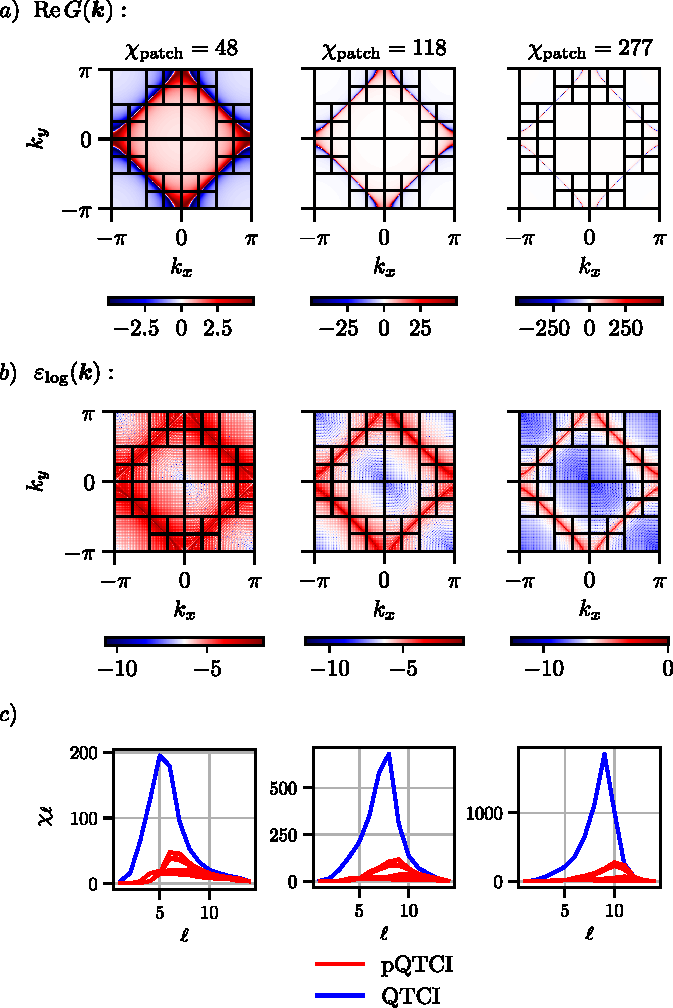
\includegraphics{figures/2DGreenErrorHeatmap.pdf}
    \caption{Patched QTCI approximation of
           \(\operatorname{Re}G(\bk)\).
           $(a)$ Heatmaps of the patched tensor train evaluated on \([-\pi,\pi]^{2}\) for bond–dimension caps \(\chi_{\text{patch}}=48,118,277\) (corresponding to
           \(\delta=10^{-1},10^{-2},10^{-3}\), respectively).
           (b) Log–error \(\varepsilon(\bk)\) [\prettyref{eq:localError2DGreen}]
           for the same patched approximations. }
    \label{fig:2DGreenErrorHeatmap}
\end{figure}

Despite the fact that \(\varepsilon(\bk)\) does not drop everywhere below the target tolerance \(\tau=10^{-7}\), its \emph{spatial average} error is of that
order. For the same parameters the conventional (Q)TCI routine attains comparable accuracy, as illustrated in \prettyref{fig:TCI2DGreenerror} for
\(\delta=10^{-1}\).
\begin{figure}[ht!]
    \centering
    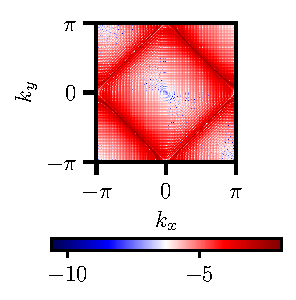
\includegraphics{figures/heatmap_TCI_error_2DGreen_ω_0.1_δ_0.1_R_15_abstol_1.0e-7_unfol_fused.pdf}
    \caption{Local error \(\varepsilon(\bk)\) for a standard QTCI approximation of \(\operatorname{Re}G(\bk)\) at \(\delta=10^{-1}\).}
    \label{fig:TCI2DGreenerror}
\end{figure}

A one–dimensional cut at \(k_{y}=\pi/2\) (\prettyref{fig:lineError2DGreen}) confirms that the patched approximation faithfully reproduces the sharp features of \(\operatorname{Re}G(\bk)\) for all three
\(\delta\) values.
\begin{figure}[ht!]
    \centering
    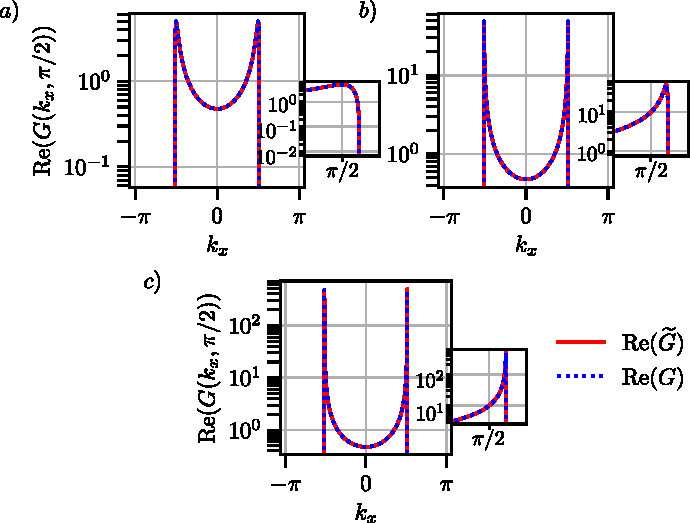
\includegraphics{figures/lineError2DGreen.pdf}
    \caption{One–dimensional slice,
           \(\operatorname{Re}G(k_{x},k_{y}=\pi/2)\),
           comparing the patched approximation (solid red) with the exact
           function (dotted blue) for
           \(\delta=10^{-1}\) (a),
           \(\delta=10^{-2}\) (b),
           and \(\delta=10^{-3}\) (c).}
    \label{fig:lineError2DGreen}
\end{figure}

We now benchmark patched QTCI (pQTCI) against the standard QTCI routine for
the Green’s function introduced above.  For each broadening
\(\delta\in\{10^{-1},10^{-2},10^{-3}\}\) we measure

\begin{itemize}
  \item the \emph{run time} on an Intel\textsuperscript{\textregistered}
        Xeon\textsuperscript{\textregistered} W-2245 CPU @ 3.90 GHz, and
  \item the \emph{memory footprint}, here defined as the total number of
        floating-point parameters in all patches
        \(\operatorname{Re}\widetilde{G}^{p_{1},\dots,p_{\bar\ell}}\).
\end{itemize}

The tensor \(\operatorname{Re}G_{\bsigma}\) is discretised with
\(\mathcal R=15\) bits per momentum component and approximated to a tolerance
\(\tau=10^{-7}\).  We scan the bond–dimension cap
\(\chi_{\text{patch}}\) and compare fused and interleaved bit orderings.

\begin{figure}[htbp]
    \centering
    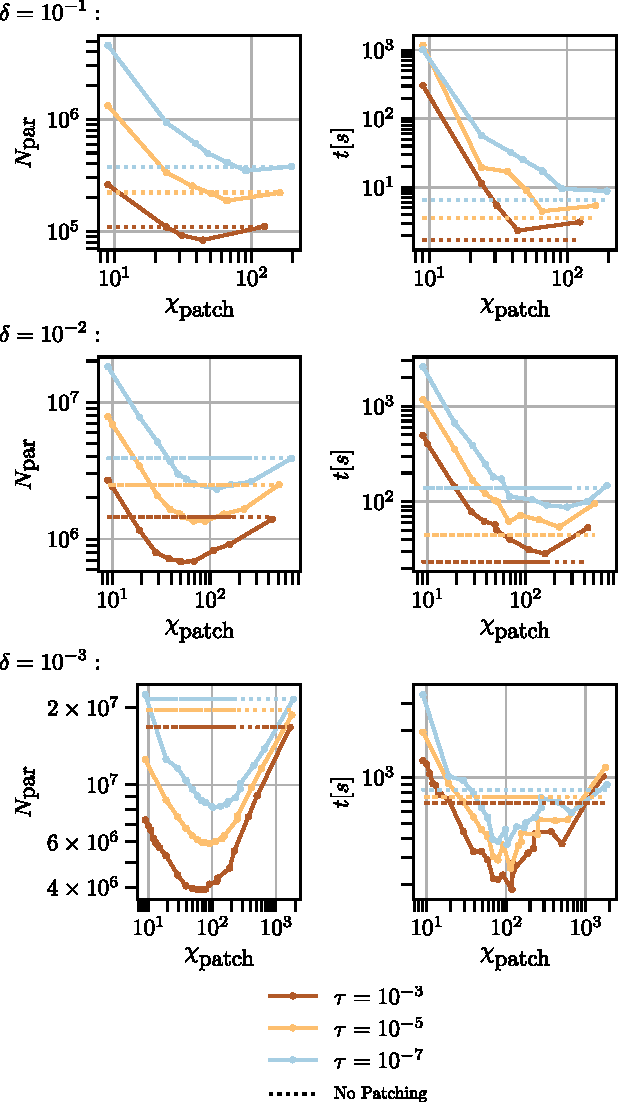
\includegraphics{figures/2DGreenMemoryTimeFused.pdf}
    \caption{ \textbf{Fused ordering.} Total parameter count (left) and CPU run time (right) versus bond-cap \(\chi_{\text{patch}}\) for \(\delta=10^{-1},10^{-2},10^{-3}\). Dotted lines show the corresponding standard-QTCI values. }
    \label{fig:memoryTime2DGreenFused}
\end{figure}

\begin{figure}[htbp]
    \centering
    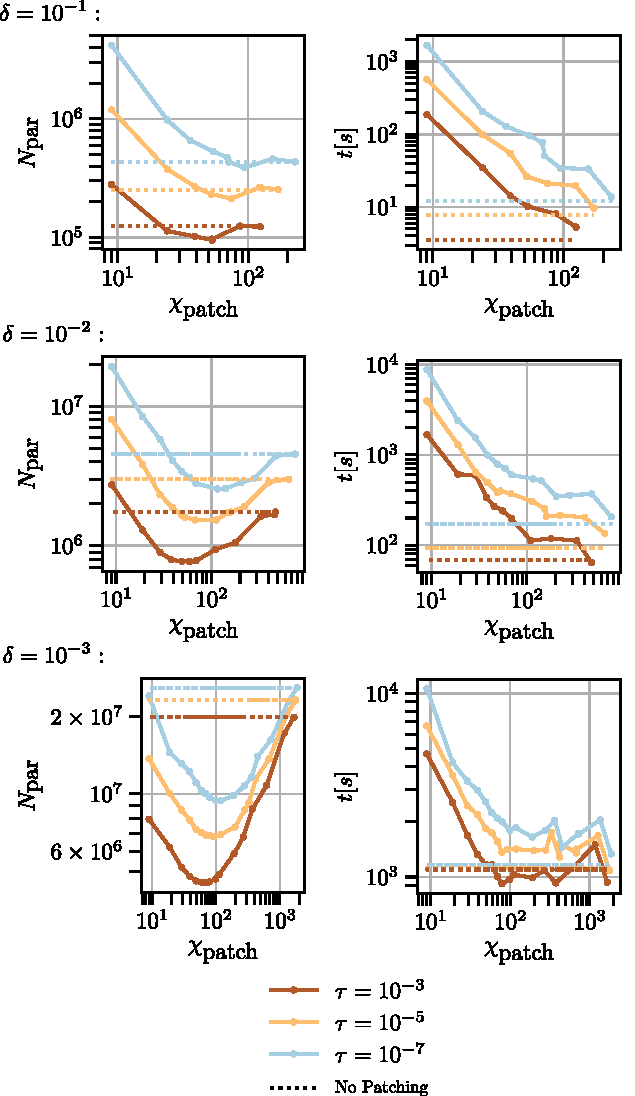
\includegraphics{figures/2DGreenMemoryTimeInterleaved.pdf}
    \caption{\textbf{Interleaved ordering.}
    Same data as \prettyref{fig:memoryTime2DGreenFused}, but with
    interleaved bit strings.}
    \label{fig:memoryTime2DGreenInterleaved}
\end{figure}

Figures~\ref{fig:memoryTime2DGreenFused}–
\ref{fig:memoryTime2DGreenInterleaved} reveal three main trends:

\begin{enumerate}
\item For \(\delta=10^{-2}\) and \(10^{-3}\) the patched routine beats standard QTCI in memory requirements. CPU rutime is smaller only with fused intex ordering. The advantage grows as the poles sharpen (smaller~\(\delta\)).

\item Each curve exhibits an optimal
      \(\chi_{\text{patch}}^{\mathrm{best}}\): setting the cap too low triggers the ``overpatching'' effect discussed in
      \prettyref{sec:patchingCost}, inflating the patch count without reducing ranks further.

\item Surprisingly, the fused ordering runtimes performs better than the interleaved one, although,in most cases, both respect the theoretical patch bounds of \prettyref{eq:chiPatchBound} for the total number of patches $\Np$. (cf. Sec.~\ref{app:2DGreenbounds} of \prettyref{app:bounds} for more details).
\end{enumerate}

For the broadest line, \(\delta=10^{-1}\), pQTCI offers no gain—the function is already smooth enough that a single TT suffices, and the extra slicing merely adds overhead.

A global view of the “return on investment’’ is given in \prettyref{fig:deltavsMemoryTime}, which plots the ratio of plain QTCI result to the best patched result (in parameters and run time) as a function of \(\delta\).  The larger is the ratio, the greater the benefit of using pQTCI.

\begin{figure}[ht!]
    \centering
    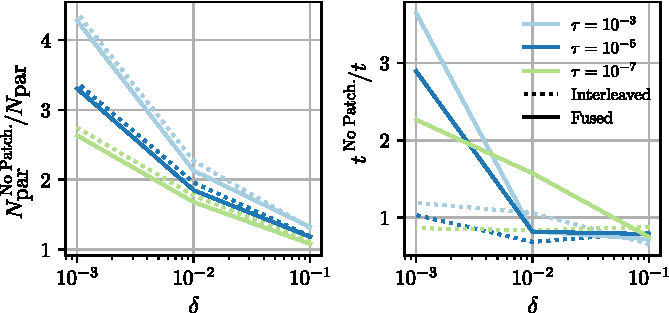
\includegraphics{figures/localisationParam2DGreen.pdf}
    \caption{Parameter and run-time ratios between the best patched approximation (at \(\chi_{\text{patch}}^{\mathrm{best}}\)) and a single-TT QTCI
    approximation, as a function of the broadening \(\delta\).} 
    \label{fig:deltavsMemoryTime}
\end{figure}

In summary, adaptively partitioning the domain allows one to focus bond dimension where it is truly needed, yielding significant savings for sharply localised Green’s functions, while incurring in overhead (``overpatching'') when the function is already smooth.

\section{Benchmarking of Patched MPO-MPO Contractions}
\label{sec:benchmarkMPOMPOContr}
Consider the two model functions 

\begin{align}
f(\bx) = \sum_{j=1}^4 e^{-(\bx - \bx_j)^2/\sigma^2_j}, \quad  
g(\bx) = \sum_{j=1}^4 e^{-|\bx - \bx'_j|/\sigma_j}, 
\label{eq:linearGauss}
\end{align}
with $\bx_j = (\cos \phi_j, \sin \phi_j )$, $\phi_j = (j-\frac{1}{2}) \frac{\pi}{2}$, $\sigma_j =  2^{-(j+1)}$, and $\bx'_j =\bx_j + (2\sigma_j,
\sigma_j)$. \prettyref{fig:factorsHeatmaps} shows heatmaps of \(f\) and \(g\).

\begin{figure}[htbp]
    \centering
    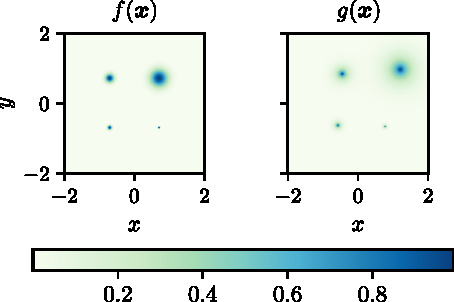
\includegraphics{figures/linearCombGauss.pdf}
    \caption{Heatmap of $f(\bx)$ and $g(\bx)$ defined in \prettyref{eq:linearGauss}.}
    \label{fig:factorsHeatmaps}
\end{figure}

We convert each function to a tensor via quantics rebasing (fused or interleaved),
\begin{equation}
    f(\bx) \mapsto \mF_{\bsigma}, \quad g(\bx) \mapsto \mG_{\bsigma}.
    \label{eq:tensorFactors}
\end{equation}
Applied to \(\mF_{\bsigma}\) and \(\mG_{\bsigma}\), the patched QTCI routine yields collections of tensor–train patches \(\{\mF^{p_{1},\dots,p_{\bar\ell}}_{\bsigma}\}\) and \(\{\mG^{p_{1},\dots,p_{\bar\ell}}_{\bsigma}\}\). We use these patch representations, after MPS-to-MPO folding (cf. \prettyref{eq:MPStoMPO}), as input for our \textit{patched MPO-MPO contraction} routines.

\subsection{Matrix multiplication}

Let the tensors \(\mF_{\bsigma}\) and \(\mG_{\bsigma}\) be stored in the \emph{interleaved} quantics format  

\[
  \bsigma
  =( \sigma_{x,1},\sigma_{y,1},\sigma_{x,2},\sigma_{y,2},\dots,
     \sigma_{x,\mathcal R},\sigma_{y,\mathcal R}),
  \qquad
  \mathcal R=17.
\]

When pQTCI is applied, the slicing (projection) order determines the resulting
patch tiling:
\begin{itemize}
  \item \textbf{Row patching:}\;
        \(p_{x,1}\!\to p_{x,2}\!\to\cdots\to p_{x,\mathcal R}\)
        (top–left panel of \prettyref{fig:patchingPatternsMatMul});
  \item \textbf{Column patching:}\;
        \(p_{y,1}\!\to p_{y,2}\!\to\cdots\to p_{y,\mathcal R}\)
        (centre–left panel);
  \item \textbf{Interleaved patching:}\;
        \(p_{x,1}\!\to p_{y,1}\!\to p_{x,2}\!\to\cdots\to p_{x,\mathcal R}\)
        (bottom–left panel).
\end{itemize}

Because pQTCI is adaptive, the actual patch pattern follows the feature structure of the functions; from left to right, each column in \prettyref{fig:patchingPatternsMatMul} correspond to the factors in \prettyref{eq:linearGauss} and their patched MPO contraction, respectively.

Each tensor‐train patch can be folded into an MPO (\prettyref{eq:MPStoMPO}) and fed to the patched MPO–MPO contraction routines.  
For instance, the two–dimensional convolution  
\begin{equation}
    h(x,y) = \int ds f(x,s)s(x,s)
\end{equation}
maps to the patched ``matrix multiplication'' 

\begin{equation}
    \mathcal{H} = \sum_{\bsigma'} \mF_{\bsigma\bsigma'}\mG_{\bsigma'\bsigma''},
\end{equation}

where only mutually compatible patch pairs need be multiplied. Although the labels “row”  and “column” may seem inverted when viewed against the two-dimensional tilings in \prettyref{fig:patchingPatternsMatMul}, they are perfectly natural in the \emph{matrix} interpretation of each tensor—where the 
$x$-bit string forms the row index and the 
$y$-bit string the row index.

\begin{figure}[htbp]
    \centering
    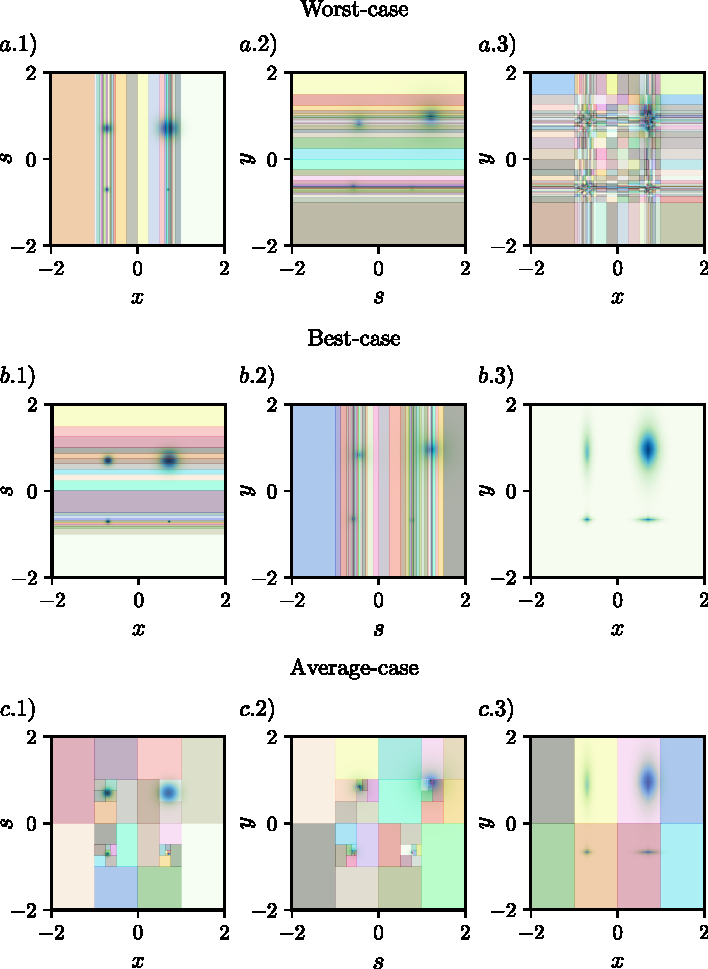
\includegraphics{figures/PatchContrResults.pdf}
    \caption{Patch tilings for the two factors \(\widetilde{\mF}\) (panels
    $a–c.1$) and \(\widetilde{\mG}\) $(a–c.2)$, together with the corresponding
    patched product \(\widetilde{\mathcal H}\) $(a–c.3)$. Rows illustrate three representative patching contraction strategies as in \prettyref{fig:2DPatchMatMul}: $(a)$ rows patching against column patching, i.e. \emph{worst‐case} in terms of contraction count;
    $(b)$ column patching against row patching — the \emph{best‐case};
   $(c)$ interleaved patching (alternating \(x\) and \(y\)) — the
    \emph{average} scenario. Each patch is rendered in a distinct colour for more clarity.}
    \label{fig:patchingPatternsMatMul}
\end{figure}

\prettyref{fig:patchingPatternsMatMul} compares the patch layouts that pQTCI produces for \(f\) and \(g\) under combinations of the three slicing orders introduced above.  
Column~$(1)$ shows the set \(\{\widetilde{\mF}^{p_{1},\dots,p_{\bar\ell}}\}\) that enters as the left factor of the convolution; column~$(2)$ shows the right–factor patches
\(\{\widetilde{\mG}^{p_{1},\dots,p_{\bar\ell}}\}\); column~$(3)$ displays the patches \(\{\widetilde{\mathcal H}^{p_{1},\dots,p_{\bar\ell}}\}\) produced by the patched MPO–MPO contraction. Colours encode individual patches, allowing one to see at a glance how the
domain is split and how the resulting product inherits the finer of the two tilings. From the two-dimensional tilings one sees that the product tensor adopts the row patching of the left factor along the $x$-direction, while its $y$-direction patching follows the column pattern of the right factor.

We now compare the patched–contraction schemes of \prettyref{fig:patchingPatternsMatMul} with a single, non-patched MPO–MPO contraction.  
\prettyref{fig:patchedMulResults} reports the wall-clock time versus the product of the  patch bond caps \(\chi_{\text{patch}, \mF}\) and  \(\chi_{\text{patch}, \mG}\)--fixed in the preliminary pQTCI runs-- for the three patch layouts, measured on an Intel\textsuperscript{\textregistered}  Xeon\textsuperscript{\textregistered} W-2245 CPU @ 3.90 GHz.
\begin{figure}[htbp]
    \centering
    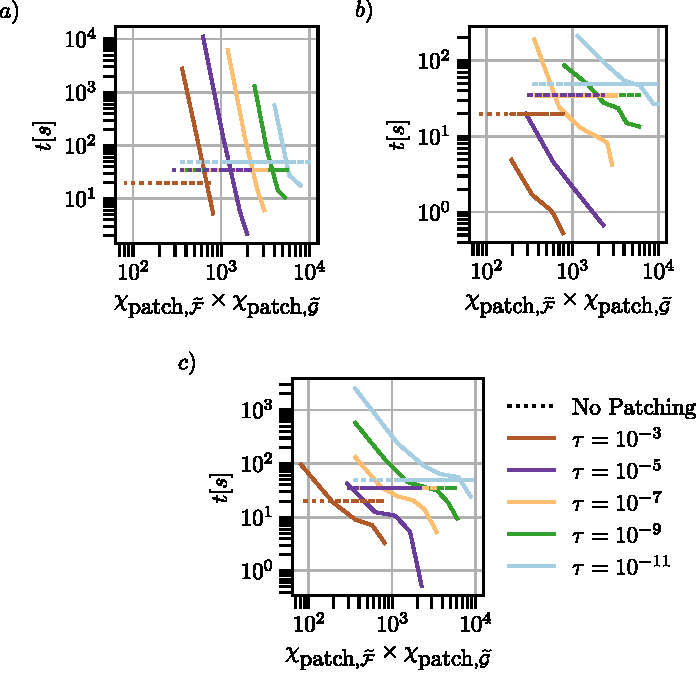
\includegraphics{figures/patchedMulResults.pdf}
    \caption{ Run-time scaling of the patched MPO–MPO contraction for the $(a)$ worst,
    $(b)$ best, and $(c)$ mixed (average) patch arrangements as in \prettyref{fig:patchingPatternsMatMul}. Dotted lines mark the reference time of a monolithic contraction with the same tolerance. }
    \label{fig:patchedMulResults}
\end{figure}

Key observations:

\begin{itemize}
    \item \emph{Worst-case layout}—column patches on both factors—exhibits the slowest scaling, consistent with the \(\mathcal N_{\text{patch}}^{2}\) contraction count predicted in \prettyref{eq:worsScaling}.
    \item For very small \(\chi_{\text{patch}}\) all three patch configurations rise again, signalling \emph{over-patching}: the initial pQTCI step subdivides \(\mF\) and \(\mG\) so aggressively that the overhead of launching thousands of tiny contractions outweighs the benefit of lower ranks.
    \item Around an intermediate, problem-dependent \(\chi_{\text{patch}}^{\mathrm{opt}}\) the patched approach becomes advantageous.  In the best-case arrangement [panel~(b)] the speed-up reaches an order of magnitude relative to the single-core baseline.
\end{itemize}

The speed-up is consistent with the limits on $\Np$ derived in Eqs~\eqref{eq:worstBound}-\eqref{eq:averageBound}; a detailed analysis is provided in Sec.\ref{sec:PatchContrbounds} of Appendix~\ref{app:bounds}.


\subsection{Element-wise multiplication}

Let \(\mF_{\bsigma}\) and \(\mG_{\bsigma}\) be represented in either the
\emph{interleaved} or \emph{fused} quantics format.  
After pQTCI compression and MPO diagonalisation
(\prettyref{eq:diagSiteTensors}), the two MPOs can be fed to the \emph{patched
element-wise contraction} routine, which produces
\begin{equation}
 \bigl(\mF\mG\bigr)_{\bsigma} = \mF_{\bsigma}\mG_{\bsigma}
\end{equation} 
i.e.\ the tensorised counterpart of the pointwise product 
\begin{equation}
    (fg)(x,y) = f(x,y)g(x,y).
\end{equation}
Knowing the analytic forms of \(f\) and \(g\), we monitor the patchwise error with the metric of \prettyref{eq:localError2DGreen} (where $\bk \to \bx$).  
\prettyref{fig:localErrorElemmul} shows the local error across the domain for a set tolerance \(\tau=10^{-7}\)—applied both in pQTCI and as the square root of thetruncation threshold in each \emph{zip-up} contraction.

\begin{figure}[htpb]
    \centering
    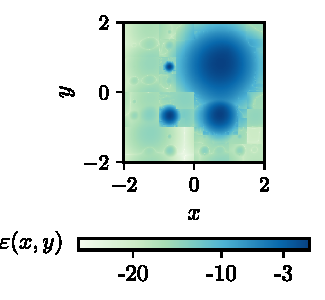
\includegraphics{figures/elemMulError.pdf}
    \caption{Pointwise error \(\varepsilon(\bx)\) of the patched element-wise product for \(\tau=10^{-7}\), $\chi_{\text{patch},\mF} = \chi_{\text{patch},\mG} = 68$ with interleaved ordering.}
    \label{fig:localErrorElemmul}
\end{figure}



Because a diagonal MPO is non-zero only on matching input/output indices, two patches contribute to the product only if they cover the \emph{same} \((x,y)\) tile.  
\prettyref{fig:patchingPatternsElemMul} illustrates this: panels $(a)$ and $(b)$ show the patch layouts of the patched tensors \(\widetilde{\mF}\) and
\(\widetilde{\mG}\); panel (c) displays the resulting patches of the product, which appear only where the patched in $(a)$ and $(b)$ overlap (cf.\
\prettyref{fig:patchElemContr}). The result is a patched tensor \(\widetilde{\mF\mG}\) that inherits -- in each region of the domain -- the smallest subdivision possible between the two factors.
\begin{figure}[htbp]
    \centering
    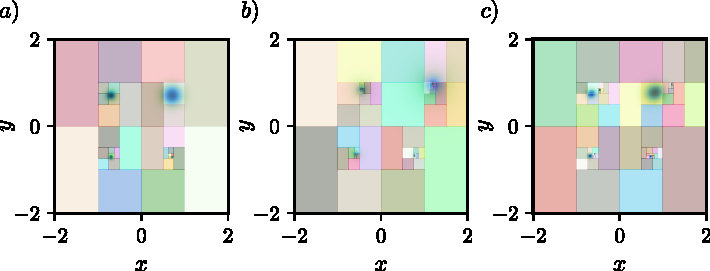
\includegraphics{figures/ElemmulResults.pdf}
    \caption{Patch tilings of $(a)$ \(\widetilde{\mF}\), $(b)$ \(\widetilde{\mG}\) and $(c)$ their patched element-wise product \(\widetilde{\mF\mG}\). Only overlapping tiles produce a non-zero result.}
    \label{fig:patchingPatternsElemMul}
\end{figure}

Element-wise multiplication enjoys the most relaxed patch-count bound (\prettyref{eq:elemMulBound}; see also
Sec.~\ref{sec:PatchContrbounds} in Appendix~\ref{app:bounds}), and the timing
data in \prettyref{fig:elemMulResults} confirm the advantage. With fused ordering the patched routine achieves up to a five-fold speed-up
over a monolithic contraction; interleaved ordering is still faster than the baseline in for some choices of $\chi_{\text{patch},\mF}$ and $\chi_{\text{patch},\mG}$, though by a smaller margin.



\begin{figure}[ht!]
    \centering
    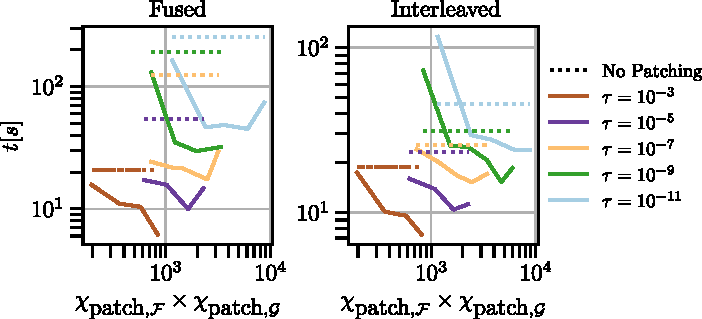
\includegraphics{figures/elemmulTimeResults.pdf}
    \caption{Runtims for patched element-wise multiplication versus the product of the bond caps \(\chi_{\text{patch},\mF}\chi_{\text{patch},\mG}\). Solid lines: patched contraction with fused or interleaved index ordering; dotted lines: reference time for a single, non-patched contraction at the same tolerance. }
    \label{fig:elemMulResults}
\end{figure}

\subsection{Adaptive matrix multiplication}


\begin{figure}[ht!]
    \centering
    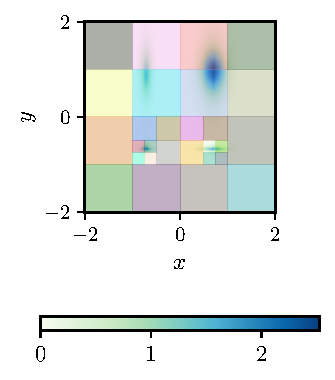
\includegraphics{figures/AdaptiveMulHeatmap.pdf}
    \caption{Heatmap + patch grid of adaptive matrix multiplication (linear combination of gaussians). }
\end{figure}

\begin{figure}[ht!]
    \centering
    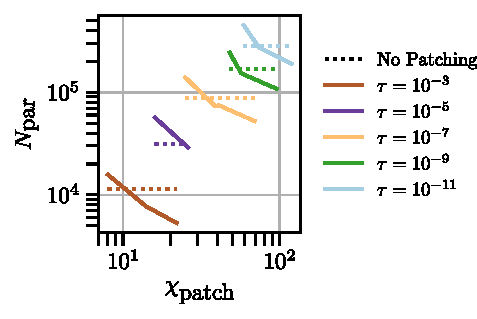
\includegraphics{figures/adaptiveMulMemory.pdf}
    \caption{Memory scaling adaptive mul}
\end{figure}




\section{Bare Susceptibility Calculation}
\label{sec:bubbleCalc}

\note{Papers}{Convolution in frequency domain \cite{Rakhuba2015}}

\begin{figure}[ht!]
    \caption{Heatmap and scheme of the global computation (TCI+QFT+ element-wise contraction + patch sum + $\textrm{QFT}^{-1}$ )}
\end{figure}

\begin{figure}[ht!]
    \caption{Memory and time scaling vs function parameter ($\beta$, $R$, $\epsilon$) comparison patch/non-patch }
\end{figure}



\section{Bethe-Salpeter equations}
\label{sec:patchBSE}

\subsection{\texttt{automul} algorithm}

\begin{figure}[ht!]
    \caption{Algorithm flowchart of matrix + element-wise multiplication\\(\texttt{automul}).}
\end{figure}

\begin{figure}[ht!]
    \caption{Heatmap of TCI and patched TCI approximation of the BSE vertices with patch grid (2D slices or multiple 2D sliced for 3D figure )}
\end{figure}

\begin{figure}[ht!]
    \caption{Memory vs patch bond dimension comparison patched/non-patched (show sub-optimal approximation)}
\end{figure}

\begin{figure}[ht!]
    \caption{N patches vs patch bond dimension with optimal number of patches reference for matrix muliplication for each BSE vertex (highlight chosen data for contraction)}
\end{figure}

\begin{figure}[ht!]
    \caption{Memory and time scaling patched/non-patched BSE contraction vs $R$ and $\epsilon$.}
\end{figure}




% \section{Gaussian Orbital Overlap}

% \note{Orbitals overlap}{Yuriel's paper on atomic bases: \cite{Jolly2024}, double-zeta calculation(?)}

% The electron repulsion integral of two GTOs is defined as

% \begin{equation}
%     \bra{\textbf{A}, \textbf{C}}\frac{1}{r_{12}}\ket{\textbf{B}, \textbf{D}} = \int_{-\infty}^\infty \text{d}^3r_1 \int_{-\infty}^\infty \text{d}^3r_2 \frac{\phi_\textbf{A}(\bm{r}_1) \phi_\textbf{B}(\bm{r}_1) \phi_\textbf{C}(\bm{r}_2) \phi_\textbf{D}(\bm{r}_2)}{|\bm{r}_1 - \bm{r}_2|}
% \end{equation}

% where the generic Cartedisan GTO can be written as

% \begin{equation}
%     \ket{\textbf{R}} = \phi_\textbf{R}(\bm{r}) = N (x - R_x)^l (y - R_y)^m (z - R_z)^n e^{-\alpha (\bm{r} - \textbf{R})^2}.
% \end{equation}
% The electron repulsion integral can be rewritten as (cf. Ref. \cite{Petersson2010}): 

% \begin{align}
%     \bra{\textbf{A}, \textbf{C}}\frac{1}{r_{12}}\ket{\textbf{B}, \textbf{D}} =& \frac{N_\textbf{A}N_\textbf{B}N_\textbf{C}N_\textbf{D} \pi^{5/2}}{\gamma_p\gamma_q\sqrt{\gamma_p + \gamma_q}} e^{\eta_p(\textbf{A} - \textbf{B})^2} e^{\eta_q(\textbf{C} - \textbf{D})^2} \times \\
%     \nonumber &\sum_{\bm{i},\bm{o},\bm{r},u}\mathcal{J}_x \sum_{\bm{j},\bm{p},\bm{s},v} \mathcal{J}_y \sum_{\bm{k},\bm{q},\bm{t},w} \mathcal{J}_z\ 2F_\nu (\eta (\textbf{P} - \textbf{Q})^2)
% \end{align}

% where

% \begin{equation} 
%     F_\nu(u) = \int_{0}^{1} \text{d}t\ t^{2\nu} e ^{-ut^2}
% \end{equation}

% is the so-called \textit{Boys function} \cite{Boys1950}.

    
% \begin{equation}
%     \begin{alignedat}{5}      
%       \textbf{P} &= \frac{1}{\gamma_p}(\alpha_1 \textbf{A} + \alpha_2 \textbf{B}) &\qquad \gamma_p &= \alpha_1 + \alpha_2 \\[6pt]
%       \textbf{Q} &= \frac{1}{\gamma_q}(\alpha_3 \textbf{C} + \alpha_4 \textbf{D}) &\qquad \gamma_q &= \alpha_3 + \alpha_4 \\[6pt]
%       \eta &= \frac{\gamma_p\gamma_q}{\gamma_p + \gamma_q}
%     \end{alignedat}
% \end{equation}
    

% \begin{figure}[ht!]
%     \caption{TCI and patched TCI approximation of the Boys function.}
% \end{figure}

% \begin{figure}[ht!]
%     \caption{3D graph of Gaussian orbitals for \ce{H2} and \ce{LiH}}
% \end{figure}

% \begin{figure}[ht!]
%     \caption{Memory and time scaling of orbital overlap compared with standard approach. }
% \end{figure}


